\chapter{Tietoturva}\label{tietoturva}

Tietoturvalla tarkoitetaan tietokonejärjestelmien ja verkkojen suojelemista elektronisten resurssien varkauksilta, ohjelmistojen ja laitteiden vahingoilta sekä tahallen aiheutetuilta häiriöiltä palvelujen toimintakyvyssä. Suojautumaan pyritään myös palvelujen väärinkäytöksiltä. Tietoturvan merkitys on kasvanut nopeasti digitalisaation myötä.~\cite{definitionofcyber}

\section{CIA-malli}\label{cia_malli}

Tärkeimpiä konsepteja tietoturvasta puhuttaessa on luottamuksellisuus, eheys sekä saatavuus. Tämän johdosta yksi tärkeimmistä malleista kuvata tietoturvan osa-alueita on CIA-malli (Confidentality, Integrity, Availability). Malli antaa viitekehyksen keskustellessa siitä, millainen jokin tietoturvauhka on. Mallin mukaisesti jokin tietoturvauhka kohdistuu aina yhteen tai useampaan CIA-mallin osa-alueista.~\cite{basicsofinformationsecurity}

\begin{figure}
\centering 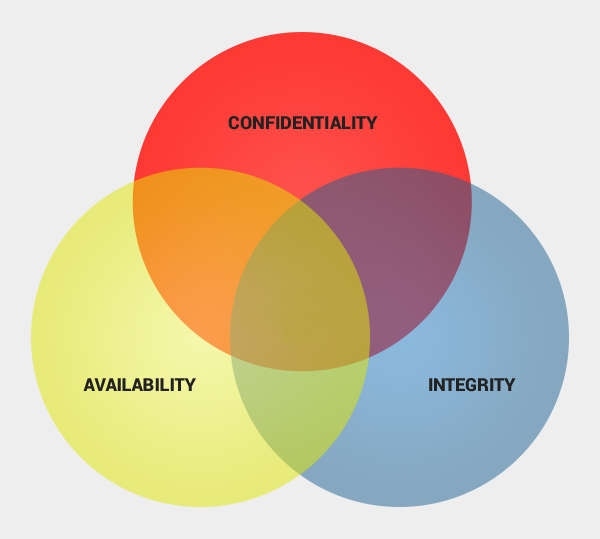
\includegraphics[width=0.5\textwidth]{kuvat/cia.png}
\caption{CIA-malli}
\label{cia} 
\end{figure}

\section{Haavoittuvuudet ja kyberhyökkäykset}\label{haavoittuvuudet_ja_kyberhyokkaykset}
Tietoturva-aukolla eli haavoittuvuudella tarkoitetaan heikkoutta tietokonejärjestelmässä, jonka avulla hyökkääjän on mahdollista päästä tekemään järjestelmässä jotakin mitä hänen ei pitäisi. Kyberhyökkäys tarkoittaa varsinaista toimenpidettä jossa hyökkääjä käyttää haavoittuvuutta päästäkseen järjestelmään.~\cite{nist}

Esittelen seuraavaksi yleisimpiä kyberhyökkäyksiä, mitä haavoittuvuutta ne hyödyntävät ja mitä CIA-mallin kohtaa ne vaarantavat. Merkitsen jokaisen esittelemäni hyökkäyksen tunnisteella ja numeroinnilla Hx, jotta niihin on helpompi palata myöhemmissä luvuissa.

\subsection{H1: Palvelunestohyökkäys}\customlabel{dos}{H1}
Palvelunestohyökkäyksen (eng. Denial of Service, DoS) tarkoitus on saada jokin verkossa oleva resurssi pois käytöstä häiritsemällä tätä internetin välityksellä. Tyypillisesti tämä saavutetaan häiritsemällä kohdetta lukuisilla palvelupyynnöillä joiden tarkoitus on saada resurssi ylikuormitettua, jonka jälkeen tavalliset resurssin käyttäjät eivät enää pääse tähän käsiksi. Palvelunestohyökkäys estää palvelun saatavuuden, joten se hyökkää CIA-mallin A-kohtaan.~\cite{nist_ddos}

Palvelintietokoneella on lukuisia rajallisia resursseja kuten kaista, levytila tai suoritinaika. Hyökkääjä voi esimerkiksi lähettää toistuvasti palvelupyyntöjä ladatakseen suuren tiedoston palvelimelta ja näin ollen tukkia kaistan tai hyökkääjä voi lähettää toistuvia palvelupyyntöjä johonkin resurssiin, jonka tietää olevan raskas suorittemelle ja näin ollen ylikuormittaa suorittimen.

Todellisuudessa harvalla hyökkääjällä on käytössään sellaisia resursseja, joilla olisi mahdollista tukkia jonkin kaupallisen toimijan palvelinresurssit. Tämän vuoksi nykyään yleisempi tapa on toteuttaa palvelunestohyökkäys on tehdä se hajautetusti (DDoS, Distibuted Denial of Service). Hajautetussa palvelunestohyökkäyksessä hyökkääjällä on käytössään useista internetiin yhdistetyistä tietokoneista muodostuva bottiverkko. Näiden tietokoneiden hallinnan hyökkääjä on saanut aikaisemmin jollakin muulla kyberhyökkäyksellä. Bottiverkossa voi olla mukana jopa satoja tuhansia tietokoneita ja tällaisen verkon haltija voi lähettää toistuvia pyyntöjä kaikilta verkon tietokoneilta samaan aikaan. Näin massiivisen verkon haltija voisi ylikuormittittaa esimerkiksi tyypillisen verkkosivuston vain yksinkertaisesti lataamalla jokaisella verkon koneella toistuvasti verkkosivustoa.~\cite{informationsecurity}

Tällaisiä ``raakaan voimaan'' perustuvia palvelunestohyökkäyksiä vastaan voi olla vaikea suojautua. Useimmat nykyaikaiset reitittimet osaavat jo jättää hyökkääjän liikenteen huomiotta, mikäli toistuvat palvelupyynnöt tulevat samasta lähteestä. Tilanne onkin toinen kun pyynnöt tulevat useista tuhansista lähteistä samaan aikaan. Tyypillisesti isoilla palveluntuottajilla on vain yksinkertaisesti niin paljon resursseja, että näitä on hyvin vaikea kenenkään tukkia. Toinen vaihtoehto on tehdä suunnitelma sen varalta, jos palvelunestohyökkäys tapahtuu. Tällaiseen suunnitelmaan voi kuulua replikaa palvelusta joka otetaan käyttöön hyökkäyksen sattuessa.

``Raa'an voiman'' käyttö palvelunestohyökkäyksissä on yksinkertaisin ja yleisin tapa, mutta palvelunestohyökkäys voidaan toteuttaa myös muilla keinoilla. Muita keinoja ovat osoitintietojen muuttaminen ja virheellisten palvelupyyntöjen lähetys sen toivossa, että palvelu kaatuu.

Kuvassa \ref{github_ddos} toistaiseksi toiseksi suurimman palvelunestohyökkäyksen piikki kaistankäytössä hyökkäyksen aikana. Hyökkäys on vuodelta 2018 ja se kohdistui Githubiin. Poikkeuksellisesti hyökkäyksessä ei käytetty bottiverkkoa vaan hyökkääjä vahvisti omia häirintäpyyntöjään tuhansilla väärinkonfiguroiduilla Memcached-palvelimilla.~\cite{wired_github_ddos}

\begin{figure}
\centering 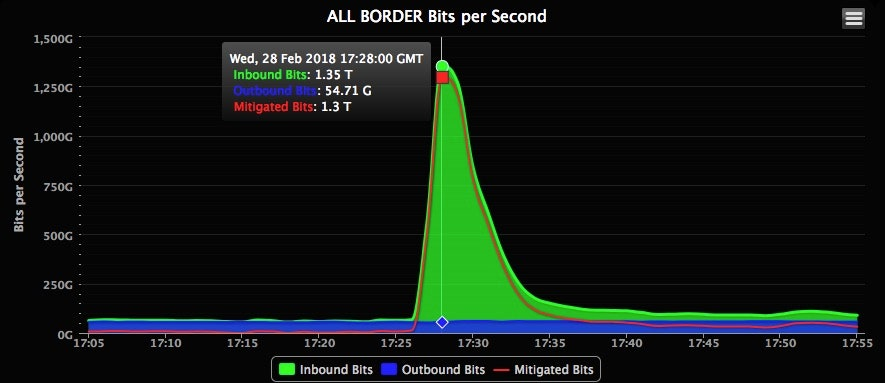
\includegraphics[width=1\textwidth]{kuvat/github_ddos.jpg}
\caption{Github DDoS 2018}
\label{github_ddos} 
\end{figure}

\subsection{H2: Takaovet}\customlabel{backdoors}{H2}
Takaovi (eng. Backdoor) on keino ohittaa järjestelmän tyypilliset autentikointimenetelmät. Tyypillisesti takaovi on tietokoneohjelma joka antaa hyökkääjälle hallinnan kohdejärjestelmästään. Esimerkiksi Linux-järjestelmässä takaovella yritetään saada tilanne aikaan jossa hyökkääjä voi kirjautua sisään kohdejärjestelmälle root-oikeuksilla käymättä kuitenkaan normaalia autentikaatioprosessia läpi. Tässä tapauksessa hyökkääjällä on täysi kontrolli kohdejärjestelmästä, joten hyökkäys voi kohdistua kaikkiin CIA-mallin osa-alueisiin.~\cite{wired_backdoor}

Takaovi asennetaan kohdetietokoneelle esimerkiksi nk.\ troijalaisen mukana. Troijalainen on viattomaksi naamioitu haittaohjelma, esimerkiksi peli, jonka mukana on kuitenkin ohjelmakoodia joka ei kuulu peliin kuten esimerkiksi takaovi.

Takaovia asennetaan myös jo muilla keinoin onnistuneen hyökkäyksen päätteeksi taatakseen hyökkääjällä pääsyn kohdejärjestelmään tulevaisuudessa.

\subsection{H3: Verkon kuuntelu}\customlabel{verkon_kuuntelu}{H3}
Verkon kuuntelu on keino salakuunnella jotakin tahoa analysoimalla verkkoliikennettä. Useimmiten liikenne on salattu joten ensin on onnistuttava murtautumaan salauksen läpi. Liikenne voi myös kulkea kaapeleita pitkin joihin pääsy on fyysisesti estetty ja itse verkkoliikenne on salaamatonta. Verkon kuuntelulla lähtökohtaisesti hyökätään CIA-mallin C-kohtaan, sillä hyökkääjä näkee tietoja jotka eivät ole hänen katseltavakseen tarkoitettu. Verkon kuuntelun tuloksena voidaan saada käsiin tietoja, joilla onnistutaan tekemään jokin muu kyberhyökkäys.

Langattomien verkkojen aikana verkon kuuntelu ei vaadi enää fyysistä pääsyä kaapeleihin, joten tarpeeksi suurella vastaanottimella hyökkääjä voi toteuttaa hyökkäyksen mistä vain. Tätä ongelmaa on korjattu vahvoilla salauksilla langattomassa verkkoliikenteessä. Varsinkin WLAN:n alkuaikoina salaukset olivat heikkoja tai niitä ei ollut lainkaan ja tämä oli suuri ongelma.

\subsection{H4: Näppäilytallennin}\customlabel{keylogger}{H4}
Näppäilytallennin (eng. Keylogger) on laite tai tietokoneohjelma joka tallentaa kaikki kohteen näppäinpainallukset ja joko lähettää ne reaaliajassa hyökkääjälle tai hyökkääjä voi hakea esimerkiksi piilotetun laitteen kohteesta. Näppäinpainallusten tallennuksella tarkoituksena on useimmiten hankkia salaiseksi tarkoitettuja tietoja, kuten salasanoja. Näppälytallennin kohdistuu CIA-mallin C-kohtaan, sillä hyökkääjä yrittää saada tietoja, joita hänen nähtäväkseen ei oltu tarkoitettu.

\subsection{H5: Koodin etäsuoritus}\customlabel{remote_code_execution}{H5}
Koodin etäsuoritus (eng. Remote Code Execution)

\subsection{H6: Eskalaatiohyökkäys}\customlabel{privilege_escalation}{H6}
Eskalaatiohyökkäys (eng. Privilege escalation)

\subsection{H7: Väsytyshyökkäys}\customlabel{bruteforce}{H7}
Väsytyshyökkäys (eng. Brute-force)

\subsection{H8: Laitteen varkaus}\customlabel{theft}{H8}
Laitteen varkaus
